\documentclass[11pt]{article}
\usepackage[margin=1in]{geometry}
\usepackage[T1]{fontenc}
\usepackage{lmodern}
\usepackage{microtype}
\usepackage{amsmath,amssymb}
\usepackage{booktabs}
\usepackage{array}
\usepackage{graphicx}
\usepackage[authoryear,round]{natbib}
\usepackage{caption}
\usepackage[section]{placeins}
\usepackage{xcolor}
\definecolor{darkblue}{rgb}{0.0,0.2,0.55}
\usepackage{xr-hyper}
\usepackage[colorlinks=true,citecolor=darkblue,urlcolor=darkblue,linkcolor=black,filecolor=black]{hyperref}
% references to the paper, built from household_pc_results.tex in this folder
\externaldocument[P-]{household_pc_results}[household_pc_results.pdf]
\captionsetup{font=small,labelfont=bf,labelsep=period}
% each figure: a takeaway headline above it and a description below it
\captionsetup[figure]{font=normalsize,position=top,justification=raggedright,singlelinecheck=false}
\newcommand{\fignote}[1]{\par\vspace{0.5em}{\small\setlength{\leftskip}{0pt}\setlength{\rightskip}{0pt}\setlength{\parfillskip}{0pt plus 1fil}#1\par}}
% let tall figures sit at the top of a text page, so that each figure stays next to the finding it shows
\renewcommand{\topfraction}{0.9}
\renewcommand{\bottomfraction}{0.8}
\renewcommand{\textfraction}{0.07}
\renewcommand{\floatpagefraction}{0.75}
\setcounter{topnumber}{2}
\setcounter{bottomnumber}{2}
\setcounter{totalnumber}{4}
\setlength{\parskip}{0.43em}
\setlength{\parindent}{0pt}
\setlength{\emergencystretch}{2em}
\newcolumntype{L}[1]{>{\raggedright\arraybackslash}p{#1}}

\title{Online Appendix\\[0.4em]
\large How Will Paid AI Spread? Evidence from Home Computers in US Households, 1984--2013}
\author{}
\date{12 November 2026}


\begin{document}
\maketitle

\noindent This online appendix accompanies the paper ``How Will Paid AI Spread? Evidence from Home Computers in US Households, 1984--2013''. Appendices A and B are in the paper, and the appendices below continue the paper's lettering, from C to I. The paper, the code, and the processed data are at \url{https://github.com/IlanStrauss/home-computer-diffusion}.

\setcounter{tocdepth}{2}
% no paragraph spacing between the entries, so the contents fit on the first page
{\setlength{\parskip}{0pt}\tableofcontents}

\clearpage
\appendix
\setcounter{section}{2}
\counterwithin{figure}{section}
\counterwithin{table}{section}
\renewcommand{\thefigure}{\thesection\arabic{figure}}
\renewcommand{\thetable}{\thesection\arabic{table}}

\section{Data details}
\label{app:data}

\subsection{What we do to the data}
\label{app:prep}

We prepare the CE files in the steps below, with \texttt{build\_ce.py} and \texttt{build\_ce\_units.py}.
\begin{enumerate}\setlength{\itemsep}{1pt}
\item Of the 671{,}792 interviews in the yearly releases of 1994 to 2013, we drop 117{,}716 repeated interviews. The CE releases its public-use interview files by year, and from the 1995 release on, each yearly release ends with the first quarter of the following year, which the next release repeats. Of the two copies of a repeated interview, we keep the copy with the appliance inventory, and the later release when both copies have the inventory.
\item We record that a household owns a computer if its appliance inventory lists a computer. The inventory almost never changes across a household's interviews.
\item We compute each household's long-run spending as four times the household's average spending per three-month interview period over all its interviews, in current dollars a year. Long-run spending leaves out vehicle purchases, spending on computers and internet service, personal insurance and pensions, and cash contributions.
\item We keep one record per household, from the household's first public interview with the appliance inventory, and we drop the 29 households with no positive long-run spending. The analysis sample then has 178{,}891 households, interviewed from January 1994 to March 2013.
\item We rescale the survey weights so that each quarter carries an equal share of its year's weight, and we scale the weights to average 1 within each year. Without the rescaling, the first quarter of 1994 would carry 51\% of that year's weight. The public files begin in that quarter, so every household then in the CE's panel enters the sample in the first quarter of 1994, at its second to fifth interview, and these households make up 5{,}190 of the 9{,}966 households of 1994. We rescale the 44 replicate weights in the same way.
\item We date each household's appliance inventory. The CE takes the inventory at the household's first interview, which is not in the public files (BLS Handbook of Methods, chapter 16), so for most households we date the inventory three months before the household's first public interview (Appendix~\ref{app:cefiles} gives the other cases). Each household gets the computer price for its inventory month.
\item We code the household traits and 29 geography groups (Section~\ref{P-sec:method} of the paper). Where the paper uses constant dollars, we divide household spending and computer prices by the PCE price index for all items (NIPA Table 2.3.4, line 1) for the household's inventory month.
\end{enumerate}

We prepare the CPS files in the steps below, with \texttt{build\_cps.py} and \texttt{cps\_extension.py}.
\begin{enumerate}\setlength{\itemsep}{1pt}
\item We keep one record per interviewed household, with the traits of the household's reference person, the person who owns or rents the home. We drop the 0.3\% of interviewed households in 1984--1993 that have no record for a reference person.
\item We record that a household owns a computer if any adult in the household answers yes.
\item We weight each household by the CPS household weight. The 1984 file has no household weight, so for 1984 we use the weight of the principal person, as the 1984 documentation advises.
\item We impute long-run spending for each household from its income bracket, with a mapping from income to spending that we estimate in the CE (Appendix~\ref{app:cpsmethod}). The fits use the 369{,}393 households in the eight supplements of October 1984 to October 2003 that have a known income bracket and known traits.
\end{enumerate}

\subsection{The CE files}
\label{app:cefiles}

Computer ownership is item 13 of the CE's major-appliance inventory. The public files carry the inventory from the first quarter of 1994 to the first quarter of 2013, and 97.4--99.9\% of interviews in each year from 1994 to 2012 have an inventory record. Across consecutive interviews of the same household, computer ownership changes in 42 of 13{,}314 pairs of interviews in 1995, in 524 of 12{,}654 pairs in 1996, and in 3 of 18{,}870 pairs in 2005, and in no pair in any other year.

We date the inventory three months before the first public interview for the 131{,}758 households first seen at their second interview. For the 42{,}221 households first seen at their third to fifth interview after 1994, we date the inventory $3 \times (\text{interview number} - 1)$ months before that interview, which assumes a first interview followed by missed interviews. For the 4{,}912 households first seen at their third to fifth interview in 1994, 3{,}903 of them in the first quarter, when the public files begin, we use the month of their first record. The last two rules are assumptions. The price paid starts in 1994, so the 1{,}287 households with inventory months in late 1993 get the 1994 price paid.

The price paid comes from the CE's minor-appliance file, which records each purchase of ``computers, computer systems and related hardware for non-business use'' with its price. We set aside purchases for someone outside the household. The item includes peripherals such as printers, which the public file cannot separate, and computer accessories have their own code from the second quarter of 2011. The 2000 release has no minor-appliance file, so the 2000 price paid rests on the first quarter of 2000. Weighted by the survey weights, the median price paid is \$400 in 1994, \$214 in 2003, \$320 in 2011, \$413 in 2012, and \$333 in 2013, and the 90th percentile is \$2{,}150 in 1994 and \$1{,}174 in 2012. In these yearly values the median price paid rose by 3\% from 1994 to 2012, and the 90th percentile fell by 45\%. Section~\ref{P-sec:quality} of the paper instead reports falls of 7\% and 47\%, which compare averages over each year's households of the log price for each household's inventory month, the basis that the second stage uses. The monthly values interpolate between mid-year values (Appendix~\ref{app:pricedata}), and 35\% of the 2012 households, by weight, have inventory months in 2011, when the median was \$320. On this basis the median price paid is \$403 in 1994 and \$374 in 2012, and the 90th percentile is \$2{,}167 and \$1{,}145.

The education of the household head is coded in four groups: less than high school, high school, some college (including associate degrees), and a college degree or more. Race is white, black, or other, and a household head who reports more than one race (from the second quarter of 2003) counts as other. In the CE files for 1994 to 2013, the state is suppressed for 10--18\% of interviews.

\subsection{The CPS files}
\label{app:cpsfiles}

The CPS Computer Use supplements (October 1984, 1989, 1993, and 1997; December 1998; August 2000; September 2001; and October 2003) give household computer ownership rates of 8.2\%, 15.0\%, 23.0\%, 36.8\%, 42.3\%, 51.1\%, 56.6\%, and 61.8\%. These rates are within 0.3 percentage points of the Census Bureau's published figures (Current Population Reports P23-208, Figure 1). Interpolation between the 1989 and 1993 surveys puts the date at which the computer ownership rate passed 20\% in spring 1992 (1992.30 on a straight line, and 1992.44 on the log-odds scale, which allows an S-shaped path between surveys). Interpolation between the 1993 and 1997 surveys puts the date at which the computer ownership rate passed 30\% in late 1995 (1995.83 and 1995.96).

The CPS records family income in 14 brackets from 1984 to 2001, with a top bracket of \$75{,}000 or more, and in 16 brackets in 2003, with a top bracket of \$150{,}000 or more. The top bracket holds 2.3\% of households in 1984, 21.1\% in 2001, and 4.5\% in 2003. The share of households with no income bracket rises from 6--8\% in 1984--1993 to 19\% in 2003.

\subsection{Long-run spending and current income}
\label{app:spending}

The household model needs a measure of what a household can afford over the life of a computer, which is the household's long-run income. One year's reported income measures long-run income less well than long-run spending does. Current income moves with job loss, retirement, and the swings of bonuses and self-employment income, and 19\% of the CE households of 1994--2013 do not report a complete, positive income. Spending follows long-run income more closely than current income does \citep{friedman1957,meyer2003}, and averaging spending over a household's interviews removes part of the quarter-to-quarter noise in spending. In the CE, log long-run spending and log current income have a correlation of only 0.63 to 0.70. Among the 142{,}957 households that report both spending and a complete, positive income in 1994--2012, a probit model of computer ownership on log long-run spending fits better than a probit model on log current income in all 19 years. The McFadden $R^2$, a measure of fit for yes-or-no models, of the income probit model is 0.54 to 0.76 times that of the spending probit model (\texttt{income\_price.py}).

The choice of income measure matters more here than in most regressions, because the spending threshold is a point on the spending axis. Suppose a measure $\tilde x_{it}$ equals log long-run income plus independent noise, both normal, with reliability $\lambda$, the share of the measure's variance that is signal, and suppose that $\mu_t$ is the mean of log long-run income. Then the spending threshold estimated with $\tilde x_{it}$ is
\begin{equation}
\tilde\tau_t = \frac{\tau_t - (1 - \lambda)\,\mu_t}{\lambda}.
\end{equation}
Noise in the income measure stretches the path of the estimated spending threshold by $1/\lambda$, which scales up $b$ and $d$, and the noise adds the growth of mean income to the unexplained trend with weight $-(1-\lambda)/\lambda$. Appendix~\ref{P-app:otherchecks} of the paper shows both effects when current income replaces long-run spending.

\subsection{Low-spending students}
\label{app:students}

Households with very low spending own computers at a high rate. Log long-run spending is left-skewed in every year (skewness $-0.16$ to $-0.70$, and $-1.23$ in 2013), with excess kurtosis of 0.4 to 3.6 (7.6 in 2013). Of the 178{,}891 CE households of 1994--2013, the 1{,}132 (0.63\%) whose spending lies more than 3 standard deviations below their year's mean own computers at a rate of 65.7\%, against 59.4\% for all other households. Of these low-spending households, 82.1\% have a household head under 25 and 59.0\% live in student housing, against 9.9\% and 1.2\% of other households. The low-spending households are mostly students, whose spending understates their resources, and the students' high computer ownership at low spending distorts a probit model of computer ownership on spending.

The regressions deal with these low-spending students in two ways. The household traits that enter on the way to the extended regression include student housing and the age of the household head, and the checks drop student housing, trim spending at the 0.5th and 99.5th percentiles, and use link functions with heavier tails.

\subsection{Computer prices}
\label{app:pricedata}

The main computer price is the BEA's PCE price index for personal computers and peripheral equipment (NIPA Table 2.4.4U, line 49), and the checks use three other quality-adjusted price indexes. The BEA's PCE price index for information processing equipment (NIPA Table 2.4.4U, line 48) adds software and other information equipment to the main index. The BEA also publishes a price index for private investment in computers and peripheral equipment (NIPA Table 5.3.4, line 11), and the BLS publishes a consumer price index for all urban consumers (CPI-U) for personal computers and peripheral equipment, which starts in December 1997. Averaged over each year's households, the basis that the second stage uses, the log computer price falls from 1994 to 2012 by 3.30 under the BEA index for information processing equipment and by 2.53 under the BEA investment index, and it falls from 1999 to 2012 by 2.36 under the CPI-U (Figure~\ref{P-fig:prices} of the paper). The PCE price index for all items, the deflator for constant dollars, rose by 0.35 in logs, or 42\%, from 1994 to 2012. Monthly values of each price place each annual value at mid-year and interpolate linearly in logs between annual values.


\section{Method details}
\label{app:method}

\subsection{First stage}
\label{app:firststage}

Each geography effect $\gamma_{g,t}$ has a Normal(0, 1) prior and each trait effect has a Normal(0, $2.5^2$) prior, so the first-stage fits are penalized maximum likelihood. The priors pull the estimated effects of small groups toward zero and barely affect large groups.

The spending correction of the extended regression is regression calibration \citep[ch.~4]{carroll2006}. The correction replaces each household's measured log long-run spending with its expected true value, given the measured value, the household's other covariates, and the number of interviews over which the household's spending is averaged. The correction uses the pooled within-household variance of log quarterly spending (0.067 to 0.115 by year). The reliability of a household's long-run spending, $\lambda_i$, which is the share of its variance that is signal, averages 0.87 to 0.94 with geography alone and 0.78 to 0.89 with household traits and education.

We chose the link function, the curve that turns household spending into a probability of owning a computer, by how well each link function predicts the computer ownership of households left out of the fit (the 10-fold cross-validated log score within each year). Under the analysis plan, we would switch from the probit model only if another link function beat the probit link by more than 4 standard errors, summed over years (Table~\ref{tab:links}). The probit model does worst with geography alone, and the probit model's deficit shrinks as household traits enter. With household traits, the best link function is the robit link, a probit-like link with heavier tails, with 7 degrees of freedom \citep{liu2004,gelman2007}, which beats the probit link by 70.6 (SE 16.5). With education, no link function beats the probit link by 4 standard errors.

The rule would switch the baseline regression, and the regression with household traits but no education, to robit models. We kept the probit model throughout, so that the four CE regressions and the joint model use one link function, and we report the rule's link functions as checks. Across link functions, the change in the spending threshold from 1994 differs by at most 0.42 with geography alone, 0.39 with household traits, and 0.21 with education.

\begin{table}[!htbp]
\centering
\caption{Cross-validated log score of each link function (10-fold within each year, weighted, summed over 1994--2013): difference from the probit link, with its standard error. Higher is better.}
\label{tab:links}
\footnotesize
\begin{tabular}{lccc}
\toprule
Link & Baseline (geography) & + household traits & + education (extended) \\
\midrule
Probit & 0 & 0 & 0 \\
Logit & +273.6 (19.5) & +62.6 (15.6) & +21.9 (14.4) \\
Robit, 7 df & +281.0 (20.9) & +70.6 (16.5) & +26.9 (14.8) \\
Robit, 4 df & +411.2 (30.3) & +55.7 (24.5) & $-$25.6 (23.0) \\
Robit, 2 df & +567.5 (45.8) & $-$101.8 (39.0) & $-$289.4 (38.2) \\
\bottomrule
\end{tabular}

\end{table}

\subsection{Second stage}
\label{app:secondstage}

The priors are
\[
a \sim \text{Normal}(10, 2^2), \quad b \sim \text{Normal}(0.5, 1), \quad d \sim \text{Normal}(0, 0.2^2), \quad \omega \sim \text{Half-Normal}(0, 0.2^2).
\]
These priors are weak. Under the priors alone, the 1994 spending threshold has a 90\% range of 6.55 to 13.35, and the change in the spending threshold from 1994 to 2013 has a 90\% range of $-11.12$ to $+7.23$, against observed values of 10.81 and $-1.99$. We fit the second-stage models with brms 2.23.0 and Stan \citep{burkner2017,carpenter2017}: 4 chains of 2{,}000 warm-up and 2{,}000 kept draws, adapt\_delta 0.99, and seed 20261109. Every fit reported here passes the standard checks that the sampler has converged: $\hat R \le 1.01$, bulk and tail effective sample sizes above 400, and no divergent transitions \citep{vehtari2021}.

\subsection{Summaries of how much the computer price explains}
\label{app:summaries}

The \emph{gap from pure affordability}, $L_t = (\tau_t - \tau_{1994}) - \ell_t$, is the change in the spending threshold since 1994 that pure affordability does not account for. The share
\begin{equation}
S_t = \frac{P^A_t - \hat P_{1994}}{P_t - \hat P_{1994}}, \qquad P^A_t = \frac{\sum_i w_{it}\,\Phi\big(\hat\alpha_{1994} + \hat\beta_{1994}(x_{it} - \ell_t - 10) + \dots\big)}{\sum_i w_{it}},
\end{equation}
compares the rise in the computer ownership rate that pure affordability predicts with the actual rise. $P^A_t$ is the computer ownership rate that pure affordability predicts: $P^A_t$ applies the fitted 1994 probit model to year-$t$ households at the year-$t$ computer price. $P_t$ is the actual computer ownership rate, $\hat P_{1994}$ is the computer ownership rate that the 1994 fit predicts for 1994's households, $w_{it}$ is household $i$'s survey weight, and the dots stand for the household's geography and trait terms at their 1994 effects. $P^A_t$ is the counterfactual of a probit decomposition \citep{fairlie2005}. $S^{\text{spend}}_t$ is the same share with $\ell_t = 0$, the part of the rise due to spending growth alone. We compute $L_t$ and $S_t$ within each replicate sample, so their standard errors allow for the covariance between years.

\subsection{The CPS extension}
\label{app:cpsmethod}

The CPS records family income in brackets, so we impute long-run spending for CPS households from a mapping that we estimate in the CE \citep{skinner1987,blundell2008}. In the CE (households with complete, positive income, 1994--1998), we convert each household's income to the CPS year's dollars with the PCE price index, place the income in that year's CPS income bracket, and replace the income by the bracket's midpoint, or, for the open top bracket, by the bracket's Pareto mean, the mean implied by a Pareto distribution fitted to the top of the income distribution \citep{parker1983}. A weighted regression of log long-run spending on the log of the bracket value, its square, the household traits, and region ($R^2$ of 0.58 to 0.59, by CPS year) maps income into spending, and we apply this mapping to each CPS household.

The CPS probit model uses the CE specification without student housing, which the CPS does not record, and the CE spending thresholds in the CPS extension use the same specification. The standard errors of the CPS spending thresholds combine the uncertainty in the mapping, re-estimated with each CE replicate weight, with CPS sampling error, taken as the probit model's sandwich standard error times $\sqrt{2}$. The factor $\sqrt{2}$ assumes a design effect of 2, which means that the survey's clustered design doubles the sampling variance. We assume a design effect because the public CPS files of these years have no replicate weights or design codes.

The switch test fits all 28 spending thresholds (8 from the CPS, 20 from the CE) with separate unexplained trends before and after a switch date $t_s$:
\begin{equation}
\tau_j = a + o\,\text{CPS}_j + b\,\ell_j + d_1 \min(t_j - t_s, 0) + d_2 \max(t_j - t_s, 0) + e_j, \qquad e_j \sim \text{Normal}(0, \omega^2),
\end{equation}
with $\hat\tau_j \sim \text{Normal}(\tau_j, \text{se}_j^2)$. Here $j$ indexes spending thresholds, $t_j$ is the date of spending threshold $j$ in decimal years, $\text{CPS}_j = 1$ for CPS spending thresholds, $o$ is the CPS offset, which absorbs differences in level between the two surveys (imputed against measured spending, and CPS households against CE consumer units), and $d_1$ and $d_2$ are the unexplained trends before and after $t_s$, as yearly changes in the log spending threshold. The profit switch hypothesis predicts $b = 1$ and $d_2 = 0$ after the switch date, with firms' profits and investment at work before the switch date. We compare three models by how well each model predicts a spending threshold left out of the fit, with leave-one-out cross-validation \citep{vehtari2017}. The first model has one unexplained trend ($d_1 = d_2$), the second switches at a computer ownership rate of 20\% (1992.44), and the third switches at 30\% (1995.96). Spending thresholds whose Pareto $k$ diagnostic exceeds 0.7, a sign that the leave-one-out approximation is unreliable, are left out and the model is refitted exactly. The priors are those of the second stage, with $o \sim \text{Normal}(0, 0.5^2)$ and $d_1, d_2 \sim \text{Normal}(0, 0.2^2)$.

\subsection{The joint model}
\label{app:jointmethod}

The joint model puts the second stage inside the probit model and fits both stages at once on all 178{,}891 CE households:
\begin{equation}
\Pr(\text{own}_{it} = 1) = \Phi\big(\beta_t\,(x_{it} - (\tau_t - 10)) + \gamma_{g(i),t} + z_{it}'\delta_t\big), \qquad
\tau_t \sim \text{Normal}\big(a + b\,\ell_t + d\,(t - 1994),\ \omega^2\big).
\end{equation}
The joint model uses the specification of the extended regression (corrected spending, geography, household traits, and education), the second stage's priors on $a$, $b$, $d$, and $\omega$, a prior $\beta_t \sim \text{Normal}^{+}(0.8, 0.5^2)$ on the spending slopes, and the first stage's penalties on $\gamma$ and $\delta$ as priors. The geography effects are constrained to $\sum_g \pi_g \gamma_{g,t} = 0$, so $\tau_t$ keeps its first-stage meaning. Each household's likelihood is weighted by its survey weight, scaled to average 1 within each year, which makes the likelihood a pseudo-likelihood \citep{savitsky2016}. We compute $\Phi$ with a logistic approximation \citep{bowling2009} whose largest error in probability is 0.00014.

The joint model has 984 parameters. Within each year the spending slope, the spending threshold, and the trait effects are correlated in the posterior, and these correlations slow the sampler. The sampler therefore works in rotated coordinates. In each year, the design matrix, weighted by the survey weights and stacked on the prior precision of the effects, is orthogonalized by a QR decomposition, and the coordinates are centred at that year's own penalized fit. The regression of $\tau_t$ on the computer price and the time trend is orthogonalized the same way \citep{stan2026}. These rotations are changes of variables, and the rotations leave the posterior unchanged. The fit uses CmdStan 2.39 with 4 chains of 1{,}000 warm-up and 1{,}000 kept draws, adapt\_delta 0.9, and seed 20261109, and the sampler starts near the two-stage solution with random jitter. The fit took 61 minutes on 8 threads in our run, on a laptop with a 10-core Apple M4 processor.


\section{Further estimates}
\label{app:detail}

The estimates in this appendix add detail to Sections~\ref{P-sec:main} and~\ref{P-sec:interaction} of the paper and test one restriction of the household model.

\subsection{Prices and incomes}
\label{app:pricesincomes}

The split of Section~\ref{P-sec:split} of the paper uses the baseline regression. The baseline regression rests on observed long-run spending, which places every household on one spending scale, and its predicted computer ownership rate differs from the observed rate by at most 0.6 percentage points in any year from 1994 to 2012. A 10\% rise in every household's spending raised the computer ownership rate 1.98 to 2.03 times as much as a 10\% fall in the computer price did, in every year from 1994 to 2012. That ratio is the exchange rate between household spending and the computer price in equation~\eqref{P-eq:channels} of the paper. The rise in spending moves every household 0.095 along the log spending axis, while the fall in the computer price moves the spending threshold by $b \times 0.105 = 0.047$.

General inflation raises household budgets and the prices of other goods alike. Inflation of this kind does not make a computer cheaper relative to other goods, and it does not raise what households can afford, so the split uses constant dollars. From 1994 to 2012 the PCE price index for all items rose by 0.35 in logs. In constant dollars the log quality-adjusted computer price fell by 4.37 (by 4.02 in current dollars), to 1/79 of its 1994 level. Median long-run spending rose by 0.13 in logs, from \$19{,}200 to \$21{,}900 a year in 1994 dollars, or by 0.48 in logs in current dollars, to \$31{,}000.

Starting from the 1994 spending threshold and spending slope, the fall in the computer price alone, through $b$, would have raised the computer ownership rate by 53.0 percentage points by 2012 with the 1994 distribution of spending (Figure~\ref{P-fig:paths} of the paper). The growth of household spending alone would have raised the computer ownership rate by 3.3 points at the 1994 computer price. Together, the fall in the computer price and the growth of household spending raise the computer ownership rate by 55.8 points, close to the rise of 56.9 points in the model's predicted computer ownership rate. The difference between 55.8 and 56.9 points comes from the unexplained trend, the 2012 year-specific deviation, and the change in the spending slope. Each of the two changes adds less once the other change has happened, because fewer non-owners remain near the spending threshold. The fall in the computer price adds 52.5 points with 2012 spending, and spending growth adds 2.8 points at the 2012 computer price. Averaging each change's contribution over the two orders gives the Shapley split of 52.8 and 3.1 points.

The same split holds in logs for the median household. From 1994 to 2012 the gap between the median household's log spending and the log spending threshold widened by 1.97 through the computer price ($b \times 4.37$) and by 0.13 through the household's own spending, so 6\% of the widening came from spending. In current dollars, which count the 0.35 of general inflation as spending growth, the Shapley split gives the computer price 81\% and household spending 19\% of the 1994--2012 rise in the computer ownership rate that prices and incomes explain, and 77\% to 84\% and 16\% to 23\% with $b$ at either end of its 90\% interval.

\subsection{The price paid}
\label{app:pricepaid}

Like the main computer price, each price paid is the average, over each year's households, of the log price for each household's inventory month, and Appendix~\ref{app:cefiles} gives the yearly values. Under the median price paid, the computer price explains only 0.05 to 0.07 of the fall of 1.45 to 2.24 in the log spending threshold from 1994 to 2012, and the unexplained trend explains almost all of the rest: $d = -0.087$ in the baseline regression and $-0.123$ $[-0.134, -0.111]$ in the extended regression, a fall in the spending threshold of 8--12\% a year that the price paid does not account for (Table~\ref{P-tab:concepts} of the paper).

\subsection{Income fifths}
\label{app:fifths}

From 1994 to 2003 the largest gain in computer ownership was in the fourth fifth from the bottom, whose computer ownership rate rose from 31.1\% to 78.1\%, or by 47 percentage points. From 2003 to 2012 the largest gain was in the second fifth from the bottom, from 46.5\% to 71.8\%, or by 25 points. In the household model, the rise in a household's probability of owning a computer from a 10\% fall in the computer price peaked at the 17th percentile of long-run spending in 2003 and at the 4th percentile in 2012. At the median household, that rise was 1.17 percentage points in 1994 and 0.95 points in 2012.

\subsection{No other interaction between the computer price and income}
\label{app:nointeraction}

The household model allows no other interaction between the computer price and household income. The computer price and household spending enter the household model only through $x_{it} - b\,\ell_t$, so a fall in the computer price is worth the same rise in spending at every level of income. If the response to the computer price depended on income in some other way, for example through a term $\eta\,x_{it}\,\ell_t$ inside $\Phi$, the spending slope, which is the coefficient on log spending inside $\Phi$, would change as the computer price fell, from $1/\sigma$ to $1/\sigma + \eta\,\ell_t$. Computer prices vary only by year, so a spending slope that stays fixed while the computer price falls is the test of this restriction.

We regress $\hat\beta_t$ on $\ell_t$ over 1994--2012 by weighted least squares, with weights $1/\text{se}(\hat\beta_t)^2$ and standard errors scaled up by the residual scatter where the scatter exceeds the replicate errors. Over the 4.02 fall in the log computer price, the estimated change in the spending slope is $-2.9\%$, $-4.6\%$, $-1.8\%$, and $-0.7\%$ of the mean spending slope in the four CE regressions, from the baseline to the extended regression. Every 90\% interval lies between $-12.3\%$ and $+10.4\%$. The data show no interaction beyond the one that the household model builds in, so \emph{a fall in the computer price was worth the same rise in spending at every level of income}.

\subsection{Yearly spending thresholds}
\label{app:thresholdtable}

Table~\ref{tab:thresholds} gives the yearly spending thresholds and spending slopes of the four CE regressions, from the baseline regression to the extended regression.

\begin{table}[!htbp]
\centering
\caption{Yearly spending thresholds $\hat\tau_t$, the log long-run spending at which a household with average location and traits has a 50\% chance of owning a computer (replicate standard errors), and spending slopes $\hat\beta_t$, from the baseline regression to the extended regression. $\ell_t$ is the main log computer price relative to 1994. 2013 has the first quarter only.}
\label{tab:thresholds}
\resizebox{\textwidth}{!}{\scriptsize
\begin{tabular}{rrrrcccccccc}
\toprule
Year & Households & Own (\%) & $\ell_t$ & \multicolumn{2}{c}{Baseline} & \multicolumn{2}{c}{+ corrected spending} & \multicolumn{2}{c}{+ household traits} & \multicolumn{2}{c}{+ education (extended)} \\
\cmidrule(lr){5-6}\cmidrule(lr){7-8}\cmidrule(lr){9-10}\cmidrule(lr){11-12}
 & & & & $\hat\tau_t$ (SE) & $\hat\beta_t$ & $\hat\tau_t$ (SE) & $\hat\beta_t$ & $\hat\tau_t$ (SE) & $\hat\beta_t$ & $\hat\tau_t$ (SE) & $\hat\beta_t$ \\
\midrule
1994 & 9,966 & 23.8 & 0.00 & 10.81 (0.05) & 0.83 & 10.72 (0.05) & 0.91 & 10.73 (0.06) & 0.96 & 11.02 (0.09) & 0.72 \\
1995 & 6,153 & 26.6 & $-$0.17 & 10.66 (0.04) & 0.87 & 10.54 (0.04) & 1.04 & 10.66 (0.05) & 0.99 & 10.95 (0.09) & 0.73 \\
1996 & 9,664 & 30.8 & $-$0.46 & 10.61 (0.03) & 0.75 & 10.53 (0.03) & 0.86 & 10.59 (0.03) & 0.90 & 10.85 (0.06) & 0.65 \\
1997 & 7,020 & 35.2 & $-$0.87 & 10.45 (0.03) & 0.83 & 10.41 (0.02) & 0.92 & 10.48 (0.04) & 0.94 & 10.69 (0.07) & 0.68 \\
1998 & 7,023 & 40.8 & $-$1.27 & 10.26 (0.02) & 0.83 & 10.23 (0.02) & 0.92 & 10.28 (0.02) & 1.01 & 10.40 (0.04) & 0.77 \\
1999 & 11,003 & 44.5 & $-$1.64 & 10.16 (0.02) & 0.83 & 10.14 (0.02) & 0.93 & 10.20 (0.02) & 0.92 & 10.27 (0.03) & 0.70 \\
2000 & 9,725 & 50.1 & $-$1.97 & 9.98 (0.02) & 0.82 & 9.98 (0.02) & 0.92 & 10.02 (0.02) & 0.96 & 10.01 (0.02) & 0.72 \\
2001 & 9,436 & 56.9 & $-$2.28 & 9.76 (0.04) & 0.79 & 9.80 (0.04) & 0.89 & 9.83 (0.02) & 0.94 & 9.74 (0.03) & 0.69 \\
2002 & 9,969 & 60.3 & $-$2.58 & 9.67 (0.04) & 0.82 & 9.71 (0.04) & 0.93 & 9.73 (0.03) & 0.97 & 9.62 (0.04) & 0.76 \\
2003 & 10,246 & 64.2 & $-$2.83 & 9.45 (0.08) & 0.70 & 9.52 (0.07) & 0.79 & 9.46 (0.06) & 0.74 & 9.18 (0.10) & 0.52 \\
2004 & 9,936 & 67.9 & $-$3.00 & 9.45 (0.06) & 0.84 & 9.52 (0.05) & 0.94 & 9.48 (0.05) & 0.92 & 9.28 (0.08) & 0.71 \\
2005 & 13,743 & 68.5 & $-$3.15 & 9.44 (0.04) & 0.78 & 9.52 (0.04) & 0.88 & 9.52 (0.04) & 0.94 & 9.28 (0.07) & 0.71 \\
2006 & 9,248 & 71.6 & $-$3.33 & 9.38 (0.06) & 0.77 & 9.47 (0.06) & 0.86 & 9.38 (0.06) & 0.85 & 8.98 (0.11) & 0.60 \\
2007 & 8,680 & 73.9 & $-$3.46 & 9.41 (0.07) & 0.85 & 9.50 (0.06) & 0.94 & 9.42 (0.06) & 0.95 & 9.08 (0.11) & 0.70 \\
2008 & 8,976 & 75.8 & $-$3.59 & 9.35 (0.09) & 0.86 & 9.45 (0.08) & 0.95 & 9.38 (0.07) & 0.96 & 9.01 (0.13) & 0.71 \\
2009 & 9,098 & 77.3 & $-$3.73 & 9.17 (0.09) & 0.78 & 9.28 (0.08) & 0.87 & 9.24 (0.06) & 0.93 & 8.88 (0.10) & 0.70 \\
2010 & 9,214 & 79.3 & $-$3.83 & 9.12 (0.09) & 0.81 & 9.23 (0.08) & 0.91 & 9.25 (0.06) & 1.03 & 8.90 (0.10) & 0.78 \\
2011 & 8,809 & 80.4 & $-$3.92 & 9.12 (0.10) & 0.83 & 9.24 (0.09) & 0.92 & 9.13 (0.07) & 0.95 & 8.75 (0.12) & 0.73 \\
2012 & 8,779 & 80.5 & $-$4.02 & 9.16 (0.08) & 0.84 & 9.27 (0.07) & 0.94 & 9.13 (0.08) & 0.94 & 8.78 (0.15) & 0.72 \\
2013 & 2,203 & 80.6 & $-$4.08 & 8.82 (0.22) & 0.65 & 8.99 (0.19) & 0.74 & 8.71 (0.27) & 0.70 & 8.10 (0.70) & 0.50 \\
\bottomrule
\end{tabular}
}
\end{table}

\section{The CPS and the test for a switch in detail}
\label{sec:cpsfull}

This appendix gives the CPS spending thresholds, compares the CPS spending thresholds with the CE spending thresholds, and reports the switch test in full. Appendix~\ref{app:cpsmethod} describes the method, and Appendix~\ref{P-sec:cps} of the paper summarizes the results.

\paragraph{The CPS spending thresholds.} Table~\ref{tab:cps} gives the CPS spending thresholds. The CPS spending thresholds barely move from 1984 to 1989 (11.34 to 11.32), while the log main computer price falls by 0.66, a fall of about half in the computer price. The CPS spending thresholds then fall steadily, to 9.70 in 2003. The 1984 and 1989 spending thresholds are the least precise, with standard errors of 0.131 and 0.115, almost all of which is CPS sampling error.

The CPS spending thresholds do not match the CE spending thresholds in the years that both surveys cover (Table~\ref{tab:validation} and Figure~\ref{fig:cps}). From 1997 to 2003 the CPS spending thresholds fall by 0.67, against 1.38 for the CE spending thresholds, and the gap between the CPS and CE spending thresholds runs from $-0.18$ to $+0.52$, or $-2.9$ to $+4.9$ standard errors. Applying the CPS imputation to CE households shows why the two surveys differ. The spending thresholds of CE households with imputed spending fall by 0.96 from 1997 to 2003, against 1.41 with the same households' corrected spending. The imputation compresses the path of the spending threshold by about a third, toward the middle of the spending distribution.

For a normally distributed $x$ with mean $\mu$ and standard deviation $\sigma_x$, the spending threshold is
\begin{equation}
\tau = \mu - \Phi^{-1}(P)\,\sqrt{1/\beta^2 + \sigma_x^2},
\end{equation}
where $P$ is the computer ownership rate. Imputed spending has a smaller spread and a steeper spending slope than corrected spending ($\hat\beta$ of 0.81 to 0.88, against 0.58 to 0.67). These two changes do not offset each other, as they would under regression calibration, so the distance between the spending threshold and mean spending shrinks. The compression vanishes where the computer ownership rate is near 50\% (2000: 9.99 imputed, 10.00 corrected) and grows as the computer ownership rate moves away from 50\%. A rough reading, which we have not estimated, is that if the CPS path is compressed by the same third, the CPS understates the relation of the spending threshold to the computer price by the same factor.

\begin{figure}[!htbp]
\caption{Imputing spending from income compresses the path of the CPS spending thresholds, so the CPS spending thresholds fall less steeply than the CE spending thresholds}
\label{fig:cps}
\centering
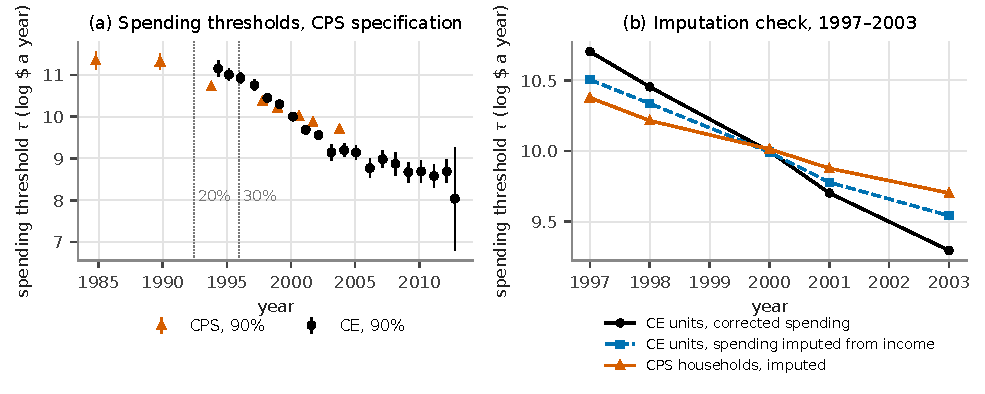
\includegraphics[width=\textwidth]{figures/cps_ce.pdf}
\fignote{(a) Spending thresholds from the CPS (imputed long-run spending, eight supplements from October 1984 to October 2003) and the CE (corrected long-run spending, 1994--2013), with the same specification and 90\% intervals, at each survey's date. (b) The imputation check, 1997--2003: spending thresholds of CE households (complete income reporters) with corrected spending and with spending imputed from their income as in the CPS, and the CPS spending thresholds.}
\end{figure}

\begin{table}[!htbp]
\centering
\caption{CPS spending thresholds (imputed long-run spending, CPS specification). Date is the survey month in decimal years. The households and computer ownership rates are those in the fit (households with a known income bracket and traits), so the computer ownership rates differ from the shares of all answering households in Appendix~\ref{app:data}. SE combines mapping and sampling error. $\ell$ is the main log computer price relative to the CE's 1994 average.}
\label{tab:cps}
\footnotesize
\begin{tabular}{rcrrcccc}
\toprule
Year & Date & Households & Own (\%) & $\hat\tau$ & SE & $\hat\beta$ & $\ell$ \\
\midrule
1984 & 1984.79 & 51,162 & 8.2 & 11.34 & 0.131 & 0.92 & 1.61 \\
1989 & 1989.79 & 50,475 & 15.2 & 11.32 & 0.115 & 0.78 & 0.95 \\
1993 & 1993.79 & 50,886 & 23.5 & 10.73 & 0.044 & 1.06 & 0.08 \\
1997 & 1997.79 & 42,458 & 38.2 & 10.38 & 0.022 & 1.10 & $-$1.12 \\
1998 & 1998.96 & 41,618 & 44.1 & 10.21 & 0.015 & 1.14 & $-$1.59 \\
2000 & 2000.62 & 40,011 & 53.4 & 10.01 & 0.011 & 1.23 & $-$2.10 \\
2001 & 2001.71 & 47,351 & 59.0 & 9.88 & 0.014 & 1.21 & $-$2.45 \\
2003 & 2003.79 & 45,432 & 64.4 & 9.70 & 0.022 & 1.09 & $-$2.95 \\
\bottomrule
\end{tabular}

\end{table}

\begin{table}[!htbp]
\centering
\caption{The CPS against the CE in the five years that both surveys cover (1997, 1998, 2000, 2001, and 2003). Left: CPS against CE spending thresholds from the same specification (CE interpolated to the CPS month). Right: CE households (complete income reporters) fitted with spending imputed from income, with corrected spending, and with observed spending (point estimates).}
\label{tab:validation}
\resizebox{\textwidth}{!}{\footnotesize
\begin{tabular}{rccccccccc}
\toprule
& \multicolumn{4}{c}{CPS against CE} & \multicolumn{5}{c}{CE households, same year} \\
\cmidrule(lr){2-5}\cmidrule(lr){6-10}
Year & CPS $\hat\tau$ & CE $\hat\tau$ & Gap & Gap/SE & $\hat\tau$ imputed & $\hat\tau$ corrected & $\hat\tau$ observed & $\hat\beta$ imputed & $\hat\beta$ corrected \\
\midrule
1997 & 10.38 & 10.56 & $-$0.18 & $-$2.9 & 10.50 & 10.70 & 10.85 & 0.88 & 0.67 \\
1998 & 10.21 & 10.32 & $-$0.11 & $-$2.9 & 10.34 & 10.45 & 10.55 & 0.84 & 0.66 \\
2000 & 10.01 & 9.85 & +0.16 & +4.1 & 9.99 & 10.00 & 9.99 & 0.83 & 0.61 \\
2001 & 9.88 & 9.61 & +0.26 & +4.9 & 9.78 & 9.70 & 9.62 & 0.82 & 0.64 \\
2003 & 9.70 & 9.18 & +0.52 & +4.9 & 9.54 & 9.30 & 9.14 & 0.81 & 0.58 \\
\bottomrule
\end{tabular}
}
\end{table}

\paragraph{A change in the unexplained trend?} Table~\ref{tab:switch} and Figure~\ref{P-fig:switch} of the paper give the results. With both surveys, which together cover 1984 to 2013, the model with a switch at a computer ownership rate of 30\% best predicts the spending thresholds left out of the fit. The 30\% switch model is ahead of the 20\% switch model by 3.8 (SE 2.1) in expected log predictive density (elpd, a measure of how well a model predicts left-out data, where higher is better), and ahead of the one-trend model by 8.7 (SE 4.5). Before late 1995 the spending threshold rose relative to the path that the computer price predicts ($d_1 = 0.052$ $[-0.007, 0.112]$), and after late 1995 the spending threshold fell relative to that path ($d_2 = -0.044$ $[-0.093, 0.008]$), a change of $-0.096$ $[-0.132, -0.060]$ a year, with $b = 0.46$ $[0.27, 0.67]$. The other BEA indexes give the same pattern. Under the 20\% switch model, all but one of the 28 spending thresholds (CPS 1993) lie inside their 90\% posterior predictive intervals.

We do not believe that the switch at 30\% is real. The switch date falls where the data change from the CPS, which supplies most of the spending thresholds before the switch date, to the CE, which supplies most of the spending thresholds after the switch date. The comparison above showed that the CPS path is compressed where the two surveys overlap, and the same compression before 1997 would make the CPS spending thresholds before the switch date fall too slowly. The spending thresholds from the two surveys also do not lie on one path. Under the main computer price, the combined fits need year-specific deviations with a standard deviation of 0.15 to 0.21, against 0.014 to 0.019 for the CPS alone. And within the CPS alone, which is the one survey that measures computer ownership consistently across both switch dates, the model with one unexplained trend predicts best, ahead of the 30\% switch model by 2.1 (SE 0.6). Within the CPS, the change in the unexplained trend is $-0.005$ $[-0.038, 0.037]$ at 30\% and $0.013$ $[-0.050, 0.079]$ at 20\%, and the one-trend model gives $b = 0.32$ $[0.15, 0.49]$ and $d = -0.012$ $[-0.062, 0.036]$.

\begin{table}[!htbp]
\centering
\caption{The switch test, CPS (October 1984 to October 2003) and CE (1994--2013): posterior medians with 90\% intervals. $d_1$ and $d_2$ are the unexplained trends before and after the switch date (yearly changes in the log spending threshold), and $o$ is the CPS offset. $\Delta\widehat{\text{elpd}}$ is the difference in expected log predictive density from the best model in its panel, with its standard error (leave-one-out, with exact refits for Pareto $k > 0.7$).}
\label{tab:switch}
\resizebox{\textwidth}{!}{\scriptsize
\begin{tabular}{lccccccc}
\toprule
Model & $b$ & $d_1$ (one trend: $d$) & $d_2$ & $d_2-d_1$ & $o$ & $\omega$ & $\Delta\widehat{\mathrm{elpd}}$ (SE) \\
\midrule
\multicolumn{8}{l}{\textit{CPS and CE spending thresholds, with a CPS offset (the approved model)}} \\
One trend & 0.46 [0.20, 0.72] & $-$0.023 [$-$0.087, +0.041] &  &  & +0.01 [$-$0.16, +0.19] & 0.212 & $-$8.7 (4.5) \\
Switch at 20\% & 0.39 [0.17, 0.61] & +0.065 [$-$0.004, +0.134] & $-$0.056 [$-$0.110, +0.001] & $-$0.121 [$-$0.176, $-$0.064] & +0.04 [$-$0.11, +0.18] & 0.169 & $-$3.8 (2.1) \\
Switch at 30\% & 0.46 [0.27, 0.67] & +0.052 [$-$0.007, +0.112] & $-$0.044 [$-$0.093, +0.008] & $-$0.096 [$-$0.132, $-$0.060] & +0.07 [$-$0.07, +0.20] & 0.150 & 0 (best) \\
\addlinespace
\multicolumn{8}{l}{\textit{CPS spending thresholds alone (check)}} \\
One trend & 0.32 [0.15, 0.49] & $-$0.012 [$-$0.062, +0.036] &  &  &  & 0.014 & 0 (best) \\
Switch at 20\% & 0.38 [0.04, 0.75] & $-$0.005 [$-$0.065, +0.057] & +0.006 [$-$0.098, +0.122] & +0.013 [$-$0.050, +0.079] &  & 0.019 & $-$2.8 (1.4) \\
Switch at 30\% & 0.30 [0.06, 0.57] & $-$0.015 [$-$0.072, +0.047] & $-$0.020 [$-$0.095, +0.069] & $-$0.005 [$-$0.038, +0.037] &  & 0.017 & $-$2.1 (0.6) \\
\bottomrule
\end{tabular}
}
\end{table}

\section{The joint model in detail}
\label{sec:joint}

The joint model matches the two-stage estimates of the extended regression (Table~\ref{tab:joint} and Figure~\ref{fig:joint}). The joint model gives $b = 0.60$ $[0.45, 0.73]$ against 0.59 $[0.46, 0.72]$ from the two stages, and $d = -0.003$ $[-0.038, 0.028]$ against $-0.005$ $[-0.037, 0.029]$, with the same posterior correlation of $b$ and $d$ (0.97). From 1994 to 2012 the joint model's spending thresholds differ from the extended regression's first-stage spending thresholds by at most 0.07 (in 2003), or 0.65 first-stage standard errors, and the joint model's spending slopes $\beta_t$ differ from the first-stage spending slopes by at most 0.04. The differences follow each first-stage spending threshold's distance from the joint model's fitted line (correlation 0.91 over 1994--2012), because the joint model pulls the yearly spending thresholds toward its fitted line, most where the first-stage standard errors are largest. The 2013 spending threshold, which rests on one quarter of data, moves from 8.10 to 8.58, or 0.68 standard errors. Over all 1{,}027 parameters and derived quantities, $\hat R \le 1.007$, bulk and tail effective sample sizes are at least 1{,}410 and 2{,}029, and there are no divergent transitions.

The joint model's intervals for $b$ and $d$ are no narrower than the two-stage intervals. The joint model's year-specific deviations are larger ($\omega = 0.090$ against 0.062), which offsets the joint model's narrower intervals for the yearly spending thresholds. Those narrower intervals are partly an artefact.

The joint model's pseudo-likelihood understates the sampling error of the spending thresholds \citep{williams2021}. Each year's fit on its own, with households treated as independent, gives standard errors of $\tau_t$ of 0.57 to 0.96 times the replicate standard errors in 1994--2012 (median 0.75). A sandwich estimator that allows for unequal weights gives 0.65 to 1.09 times the replicate standard errors (median 0.82), so the rest of the gap reflects the survey's strata and clusters and the spending correction, which the joint model treats as known. Pooling the years toward the fitted line narrows the joint model's 90\% intervals for $\tau_t$ further, to 0.49 to 0.90 times the width of the replicate intervals. The understated sampling error also inflates $\omega$, because the joint model attributes to year-specific deviations what the replicate standard errors attribute to sampling error. The joint model's intervals therefore do not reflect the survey design, and the comparison of the joint model with the two-stage fit is a comparison of point estimates.

\begin{table}[!htbp]
\centering
\caption{The joint model against the two-stage estimates (extended regression, main computer price, CE households of 1994--2013): posterior medians with 90\% intervals. The joint model's intervals do not allow for the survey design (see text).}
\label{tab:joint}
\footnotesize
\begin{tabular}{lcc}
\toprule
Parameter & Joint model & Two-stage (extended regression) \\
\midrule
$a$ & 11.14 [11.04, 11.24] & 11.15 [11.05, 11.23] \\
$b$ & 0.60 [0.45, 0.73] & 0.59 [0.46, 0.72] \\
$d$ & $-$0.003 [$-$0.038, +0.028] & $-$0.005 [$-$0.037, +0.029] \\
$\omega$ & 0.090 [0.059, 0.139] & 0.062 [0.028, 0.108] \\
\bottomrule
\end{tabular}

\end{table}

\begin{figure}[!htbp]
\caption{The joint model gives nearly the same yearly spending thresholds as the first stage of the extended regression}
\label{fig:joint}
\centering
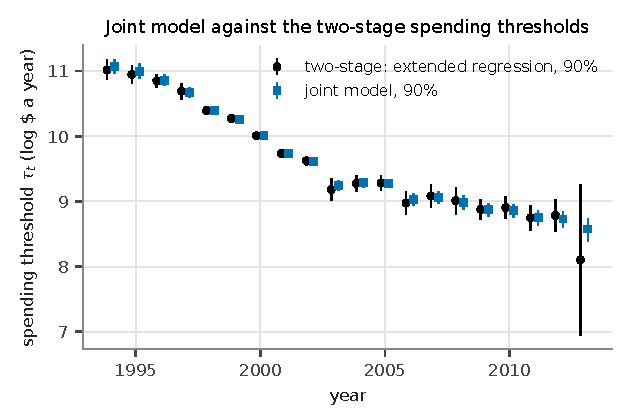
\includegraphics{figures/joint.pdf}
\fignote{Yearly spending thresholds, 1994--2013, from the joint model (posterior medians with 90\% intervals) and from the first stage of the extended regression ($\pm 1.645$ replicate standard errors). The joint model's intervals do not allow for the survey design.}
\end{figure}

\section{Departures from the analysis plan}
\label{app:deviations}

The analysis plan numbered the regressions as seven steps, and the code keeps those numbers. Step 1 is the baseline regression. Steps 2--4 add the three parts of the extended regression one at a time, steps 5 and 6 are the CPS extension, and step 7 is the joint model.

The analysis plan's cross-validation rule picks a robit model with 2 degrees of freedom for the baseline regression and a robit model with 7 degrees of freedom for the regression with household traits but no education. We kept the probit model throughout, so that every regression, the second stage, and the joint model share one link function, and we report the rule's link functions as checks. The robit link functions change the price effect little, with $b = 0.37$ $[0.30, 0.45]$ against 0.45 in the baseline regression, and $0.41$ $[0.33, 0.50]$ against 0.41 with household traits.

The analysis plan placed the date at which the computer ownership rate passed 20\% in mid-1991. Interpolation between the CPS surveys puts that date in spring 1992 (1992.30 to 1992.44), and the switch test uses 1992.44.

The full set of checks runs on the baseline and extended regressions, which bracket the two intermediate regressions, since the extended regression contains every change that the intermediate regressions make. The regression with household traits but no education has only the observed-spending and robit-model checks, and the regression with corrected spending alone has no checks of its own. The CPS spending thresholds have no link or weighting checks, since the income imputation is what limits the CPS spending thresholds.

The CPS sampling error assumes a design effect of 2, since the public CPS files of these years carry no replicate weights or design codes.

The analysis plan expected the imputed CPS spending thresholds to match the CE spending thresholds in the years that both surveys cover. The CPS spending thresholds do not match the CE spending thresholds (Appendix~\ref{sec:cpsfull}), so the switch test adds the CPS-alone check, and we read the combined CPS and CE results as an artefact of combining the two surveys.

The joint model samples in QR coordinates centred at each year's own fit. We made this change of variables because the direct parametrization reached the sampler's maximum tree depth in pilots on a 5\% subsample, and a pilot on all households had not finished its 300 warm-up iterations after 14 minutes. In the rotated coordinates the sampler needs 28 leapfrog steps per iteration on average, with a tree depth of at most 5. The joint model's geography prior applies to effects constrained by the pooled shares, whereas the first stage puts the same prior on unconstrained effects next to a free intercept. Each year's fit under the joint model's priors reproduces the extended regression's spending thresholds to within 0.004 in logs and the spending slopes to within 0.003, so this difference in priors is immaterial. The joint model's intervals do not allow for the survey design (Appendix~\ref{sec:joint}).

Two parts of the paper's findings are additions to the analysis plan, the split of the rise in the computer ownership rate between the computer price and household spending (Section~\ref{P-sec:split} of the paper) and the interaction of the computer price with household income (Section~\ref{P-sec:interaction} of the paper). Both parts use only estimates that the plan already produces (the baseline regression's fits and second stage), and their intervals allow for the uncertainty in $b$ only. The constant-dollar version of the second stage in the four CE regressions is also an addition. The constant-dollar version leaves the approved current-dollar estimates unchanged.

\section{Reproduction}
\label{app:repro}

\begingroup\raggedright
The code and the processed data are at \url{https://github.com/IlanStrauss/home-computer-diffusion}, together with the paper and this online appendix. The repository's \texttt{README.md} explains how to download the raw survey files and gives the full run order, and \texttt{run\_all.sh} runs every script in that order. After the build scripts, the run order is \texttt{explore\_data.py}, \texttt{link\_choice.py}, \texttt{first\_stage.py}, \texttt{second\_stage.R}, \texttt{second\_stage\_constant.R}, \texttt{income\_price.py}, \texttt{education\_raw\_gap.py}, \texttt{cps\_extension.py}, \texttt{cps\_switch.R 1992.44 1995.96}, \texttt{joint\_prepare.py}, \texttt{joint\_model.py}, and \texttt{joint\_design\_effect.py}, all in \texttt{code/}. Each script writes a log to \texttt{output/logs/}, and the estimates go to \texttt{output/results/}. Then \texttt{figures.py} and \texttt{tables.py} write the figures and tables of the paper and of this online appendix. The scripts fix their random seeds, so a run from the raw files reproduces the processed data, the estimates, and the tables exactly, except the joint model. The joint model sums its likelihood over years on parallel threads, and the order of that sum, and so its rounding, can change from run to run, so the joint model's estimates can differ in the last digit between runs. For readers who want the data without the model, \texttt{build\_combined.py} writes \texttt{households\_combined.csv.gz}, which holds the 178{,}891 CE households of January 1994 to March 2013 and the 425{,}627 CPS households of October 1984 to October 2003 in one file, with common variable names and codes and the BEA computer price index for the month of each household's computer answer.\par
\endgroup

\begingroup\raggedright
\begin{thebibliography}{99}
\bibitem[Blundell et~al.(2008)Blundell, Pistaferri, and Preston]{blundell2008} Blundell, R., L. Pistaferri, and I. Preston (2008). Consumption inequality and partial insurance. \emph{American Economic Review} 98(5), 1887--1921. \href{https://doi.org/10.1257/aer.98.5.1887}{doi:10.1257/aer.98.5.1887}.
\bibitem[Bowling et~al.(2009)Bowling, Khasawneh, Kaewkuekool, and Cho]{bowling2009} Bowling, S. R., M. T. Khasawneh, S. Kaewkuekool, and B. R. Cho (2009). A logistic approximation to the cumulative normal distribution. \emph{Journal of Industrial Engineering and Management} 2(1), 114--127. \href{https://doi.org/10.3926/jiem.2009.v2n1.p114-127}{doi:10.3926/jiem.2009.v2n1.p114-127}.
\bibitem[B{\"u}rkner(2017)]{burkner2017} B{\"u}rkner, P.-C. (2017). brms: An R package for Bayesian multilevel models using Stan. \emph{Journal of Statistical Software} 80(1), 1--28. \href{https://doi.org/10.18637/jss.v080.i01}{doi:10.18637/jss.v080.i01}.
\bibitem[Carpenter et~al.(2017)]{carpenter2017} Carpenter, B., A. Gelman, M. D. Hoffman, D. Lee, B. Goodrich, M. Betancourt, M. Brubaker, J. Guo, P. Li, and A. Riddell (2017). Stan: A probabilistic programming language. \emph{Journal of Statistical Software} 76(1), 1--32. \href{https://doi.org/10.18637/jss.v076.i01}{doi:10.18637/jss.v076.i01}.
\bibitem[Carroll et~al.(2006)Carroll, Ruppert, Stefanski, and Crainiceanu]{carroll2006} Carroll, R. J., D. Ruppert, L. A. Stefanski, and C. M. Crainiceanu (2006). \emph{Measurement Error in Nonlinear Models: A Modern Perspective}, 2nd ed. Boca Raton: Chapman and Hall/CRC. \href{https://doi.org/10.1201/9781420010138}{doi:10.1201/9781420010138}.
\bibitem[Fairlie(2005)]{fairlie2005} Fairlie, R. W. (2005). An extension of the Blinder-Oaxaca decomposition technique to logit and probit models. \emph{Journal of Economic and Social Measurement} 30(4), 305--316. \href{https://doi.org/10.3233/JEM-2005-0259}{doi:10.3233/JEM-2005-0259}.
\bibitem[Friedman(1957)]{friedman1957} Friedman, M. (1957). \emph{A Theory of the Consumption Function}. Princeton: Princeton University Press.
\bibitem[Gelman and Hill(2007)]{gelman2007} Gelman, A., and J. Hill (2007). \emph{Data Analysis Using Regression and Multilevel/Hierarchical Models}. Cambridge: Cambridge University Press. \href{https://doi.org/10.1017/CBO9780511790942}{doi:10.1017/CBO9780511790942}.
\bibitem[Liu(2004)]{liu2004} Liu, C. (2004). Robit regression: A simple robust alternative to logistic and probit regression. In A. Gelman and X.-L. Meng (eds.), \emph{Applied Bayesian Modeling and Causal Inference from Incomplete-Data Perspectives}, 227--238. Chichester: Wiley. \href{https://doi.org/10.1002/0470090456.ch21}{doi:10.1002/0470090456.ch21}.
\bibitem[Meyer and Sullivan(2003)]{meyer2003} Meyer, B. D., and J. X. Sullivan (2003). Measuring the well-being of the poor using income and consumption. \emph{Journal of Human Resources} 38 (Supplement), 1180--1220. \href{https://doi.org/10.2307/3558985}{doi:10.2307/3558985}.
\bibitem[Parker and Fenwick(1983)]{parker1983} Parker, R. N., and R. Fenwick (1983). The Pareto curve and its utility for open-ended income distributions in survey research. \emph{Social Forces} 61(3), 872--885. \href{https://doi.org/10.1093/sf/61.3.872}{doi:10.1093/sf/61.3.872}.
\bibitem[Savitsky and Toth(2016)]{savitsky2016} Savitsky, T. D., and D. Toth (2016). Bayesian estimation under informative sampling. \emph{Electronic Journal of Statistics} 10(1), 1677--1708. \href{https://doi.org/10.1214/16-EJS1153}{doi:10.1214/16-EJS1153}.
\bibitem[Skinner(1987)]{skinner1987} Skinner, J. (1987). A superior measure of consumption from the Panel Study of Income Dynamics. \emph{Economics Letters} 23(2), 213--216. \href{https://doi.org/10.1016/0165-1765(87)90042-5}{doi:10.1016/0165-1765(87)90042-5}.
\bibitem[Stan Development Team(2026)]{stan2026} Stan Development Team (2026). \emph{Stan User's Guide}, version 2.39, section on the QR reparameterization. \url{https://mc-stan.org/docs/}.
\bibitem[Vehtari et~al.(2017)Vehtari, Gelman, and Gabry]{vehtari2017} Vehtari, A., A. Gelman, and J. Gabry (2017). Practical Bayesian model evaluation using leave-one-out cross-validation and WAIC. \emph{Statistics and Computing} 27(5), 1413--1432. \href{https://doi.org/10.1007/s11222-016-9696-4}{doi:10.1007/s11222-016-9696-4}.
\bibitem[Vehtari et~al.(2021)Vehtari, Gelman, Simpson, Carpenter, and B{\"u}rkner]{vehtari2021} Vehtari, A., A. Gelman, D. Simpson, B. Carpenter, and P.-C. B{\"u}rkner (2021). Rank-normalization, folding, and localization: An improved $\widehat{R}$ for assessing convergence of MCMC. \emph{Bayesian Analysis} 16(2), 667--718. \href{https://doi.org/10.1214/20-BA1221}{doi:10.1214/20-BA1221}.
\bibitem[Williams and Savitsky(2021)]{williams2021} Williams, M. R., and T. D. Savitsky (2021). Uncertainty estimation for pseudo-Bayesian inference under complex sampling. \emph{International Statistical Review} 89(1), 72--107. \href{https://doi.org/10.1111/insr.12376}{doi:10.1111/insr.12376}.
\end{thebibliography}
\endgroup

\end{document}
